%% LyX 2.1.2.2 created this file.  For more info, see http://www.lyx.org/.
%% Do not edit unless you really know what you are doing.
\documentclass[english]{article}
\usepackage[T1]{fontenc}
\usepackage[latin9]{inputenc}
\usepackage{geometry}
\geometry{verbose,tmargin=1cm,bmargin=2cm,lmargin=2cm,rmargin=2cm}
\usepackage{float}
\usepackage{caption}
\usepackage{subcaption}
\usepackage{amsmath}
\usepackage{amssymb}
\usepackage{graphicx}
\usepackage{xcolor}
\usepackage{esint}

% Misc
\newcommand{\todo}[1]{}
\renewcommand{\todo}[1]{{\color{red} TODO\@: {#1}}}

\makeatletter

%%%%%%%%%%%%%%%%%%%%%%%%%%%%%% LyX specific LaTeX commands.
%% A simple dot to overcome graphicx limitations
\newcommand{\lyxdot}{.}

\makeatother

\usepackage{babel}

\begin{document}

\title{Firefly Monte Carlo: Exact MC with data subsets}
\author{Feynman Liang, Max Chamberlin, Kai Xu}
%
\maketitle

\tableofcontents

\section{Introduction}

Many methods in Bayesian inference involve computing the likelihood
$L(\theta)$ of parameters $\theta$ over iid observations
$X=\{x_{n}\}_{n=1}^{N}$, defined as

\[
L(\theta)=P(X|\theta)=\prod_{n=1}^{N}P(x_{n}|\theta)=\prod_{n=1}^{N}L_{n}(\theta)
\]

For example, Monte Carlo Markov Chain (MCMC) are a class of methods often
used to sample posterior distributions $P(\theta | X)$ with intractable
partition functions $Z = \int P(X|\theta) P(\theta) d\theta$.
When performing Metropolis-Hastings MCMC, at each iteration we need to compute
the acceptance probability

\[
A(\theta'|\theta)=\min\left\{ 1,\frac{q(\theta|\theta')L(\theta')P(\theta')}{q(\theta'|\theta)L(\theta)P(\theta)}\right\}
\]

This means that each iteration requires at least one evaluation $L(\theta')$
of the likelihood over all $N$ points ($L(\theta)$ can be cached from the
prior iteration). Unfortunately, in the era of ``Big Data''
$N$ may be on the order of petabytes and computing $L(\theta)$ at
each iteration may be prohibitively expensive.

\subsubsection*{Rationale for selecting the paper: }

We chose FlyMC because of the ubiquity of MCMC sampling methods which
see use not just in the fields of machine learning and Bayesian statistics,
but also in the fields of computational physics, biology and computational
linguistics. If large speed-ups could be obtained using the methods
expounded in FlyMC, this would be of great benefit to many different
academic communities.

Furthermore, in Bayesian statistics, the recent development of MCMC
methods has been a key step in making it possible to compute large
hierarchical models that require integrations over hundreds or even
thousands of unknown parameters, which is an exciting area of further
research. However, to make MCMC work quickly for data of the order
of that seen in the 'Big Data' era, any speed-up that is possible
would be well received.

In addition to this, FlyMC is based on a mathematically elegant idea.
The idea is that when performing inference, all that is necessary
is to \todo{finish this sentence}

\section{Theory}


The motivation for FlyMC is to achieve speed-ups over typical
MCMC by estimating a large dataset's likelihood using smaller subsets
of the data.

It also introduces auxiliary variables, which will act as indicators
for the points for which the further computation (evaluations of $L_{n}(\theta)$)
are required. This gives the motivation for the name, FlyMC, since
these auxiliary variables can be thought of as lighting up when further
likelihood evaluations are desired. Finally, with these terms in place,
an intuitive explanation of FlyMc can be given. We have a lower bound
for the likelihood, $B_{n}(\theta)$, which accounts for a large part
of the probability mass on the distribution from $\theta$. However,
there is still a difference $L_{n}(\theta)$-$B_{n}(\theta)$, which
we are uncertain of and which we would like to compute adjustments
for through sampling. FlyMCn constructs a way of sampling from this
residual probability mass, which is hopefully much smaller than $L_{n}$($\theta)$,
and so may result in large reductions in sampling time. The idea is
neatly summarised in the graph below:

\begin{figure}[H]
\begin{centering}
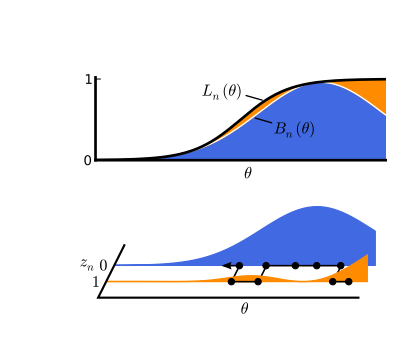
\includegraphics[scale=0.4]{Figures/gap-fig.png}
\par\end{centering}

    \protect\caption{Graphical representation of the decomposition of
    $L_n)$ into a $L_n - B_n$ part associated with bright variables $z_n = 0$
    and a $B_n$ part associated with dim variables $z_n = 0$ \cite{maclaurin2014firefly}}


\end{figure}

Firefly Monte Carly (FlyMC) is a method which addressses the computational
problem of evaluating $L(\theta)$ for a large number of data points
$N$ through exact Monte Carlo estimates of the of the full dataset
likelihood using smaller, tractable subsets. As an auxilliary variable
method, it works by augmenting the joint distribution with hidden\emph{
brightness }variables$Z=\{z_{n}\in\left\{ 0,1\right\} \}_{n=1}^{N}$to
form a \emph{complete data likelihood}

\[
P(X,Z|\theta)=\prod_{n=1}^{N}P(x_{n}|\theta)P(z_{n}|x_{n},\theta)
\]


Notice that we can recover the desired likelihoods simply through
marginalization

\[
\sum_{Z}P(X,Z|\theta)=\sum_{z_{1}}\dots\sum_{z_{N}}\prod_{n=1}^{N}P(|x_{n}|\theta)P(z_{n}|x_{n},\theta)=\prod_{n=1}^{N}P(|x_{n}|\theta)\sum_{z_{n}}P(z_{n}|x_{n},\theta)=L(\theta)
\]


In FlyMC, the brightness variables are chosen to have Bernoulli distribution

\begin{equation}
P(z_{n}|x_{n},\theta)=\left(\frac{L_{n}(\theta)-B_{n}(\theta)}{L_{n}(\theta)}\right)^{z_{n}}\left(\frac{B_{n}(\theta)}{L_{n}(\theta)}\right)^{1-z_{n}}\label{eq:brightness}
\end{equation}


where$B_{n}(\theta)$ is a lower bound on the likelihood satisfying

\begin{align}
 & 0\leq B_{n}(\theta)\leq L_{n}(\theta)\label{eq:bn-bound}\\
 & \prod_{n\in A}B_{n}(\theta)\text{ can be efficiently computed for any data subset }A\subset X\label{eq:bn-efficient}
\end{align}

\ref{eq:bn-bound} is required for \ref{eq:brightness} to be a valid
probability distribution. To see why \ref{eq:bn-efficient} is necessary,
consider computing the complete data likelihood

\begin{align}
P(X,Z|\theta) & =\prod_{n=1}^{N}P(x_{n}|\theta)P(z_{n}|x_{n},\theta)\nonumber \\
 & =\prod_{n=1}^{N}L_{n}(\theta)\left(\frac{L_{n}(\theta)-B_{n}(\theta)}{L_{n}(\theta)}\right)^{z_{n}}\left(\frac{B_{n}(\theta)}{L_{n}(\theta)}\right)^{1-z_{n}}\nonumber \\
 & =\prod_{x_{n}\in X_{bright}}\left(L_{n}(\theta)-B_{n}(\theta)\right)\prod_{x_{n}\in X_{dim}}\left(B_{n}(\theta)\right)\label{eq:bright-dim-decomposition}\\
 & =\prod_{n=1}^{N}B_{n}(\theta)\prod_{x_{n}\in X_{bright}}\frac{L_{n}(\theta)-B_{n}(\theta)}{B_{n}(\theta)}
\end{align}


where the bright points $X_{bright}=\{x_{n}:z_{n}=1\}$ and dim points
$X_{dim}=\{x_{n}:z_{n}=0\}$give rise to the ``Firefly'' in the
paper title. Notice that as a consequence of our choice for\ref{eq:brightness},\ref{eq:bright-dim-decomposition}
decomposes into two products where $\frac{L_{n}(\theta)-B_{n}(\theta)}{B_{n}(\theta)}$
only needs to be evaluated for $x_{n}\in X_{bright}$. By assuming
\ref{eq:bn-efficient}, the other term $\prod_{n=1}^{N}B_{n}(\theta)$
can be efficiently computed so the computational complexity is determined
by $X_{bright}$.


\subsection{Performance comparison}

Instead of evaluating $L_{n}(\theta)$ over all $N$ points, FlyMC
only evaluates the likelihood over a subset of points $X_{bright}$.
This provides a speedup of $\frac{N}{\#X_{bright}}$per iteration.
However, since the brightness variables $z_{n}$are themselves, to
understand the performance improvements we consider the expected number
of bright points $E[\#X_{bright}]$.

Note that for any point $x_{n}$,\ref{eq:brightness} implies the
probability $x_{n}$is bright is given by $\frac{L_{n}(\theta)-B_{n}(\theta)}{L_{n}(\theta)}$.
Hence, the number of bright points is given by

\begin{equation}
E[\#X_{bright}]=\sum_{n=1}^{N}E[z_{n}]=\sum_{n=1}^{N}\int P(\theta|X)\frac{L_{n}(\theta)-B_{n}(\theta)}{L_{n}(\theta)}d\theta\label{eq:num-bright}
\end{equation}


This says that the number of bright points (and hence the speedup
achieved by FlyMC) is related to the gap between the true likelihood
$L_{n}(\theta)$ and the lower bound $B_{n}(\theta)$, weighted by
the posterior $P(\theta|X)$.

This result makes intuitive sense. Consider the extreme case where
for all $n$: $B_{n}(\theta)=0$. Then $P(z_{n}=1|x_{n},\theta)=1$
so every data point is bright (i.e. $X=X_{bright}$) and \ref{eq:bright-dim-decomposition}
reduces to evaluating the full dataset likelihood $\prod_{n=1}^{N}L_{n}(\theta)$
as usual.

In the other extreme, if $B_{n}(\theta)=L_{n}(\theta)$ so all data
points are dim. At first it appears that FlyMC counterintuitively
offers a $\frac{N}{\#X_{bright}}=\frac{N}{0}=\infty$speedup. However,
considering \ref{eq:bright-dim-decomposition} reveals that what is
computed is $\prod_{n=1}^{N}B_{n}(\theta)=\prod_{n=1}^{N}L_{n}(\theta)$,
which by assumption \ref{eq:bn-efficient}can be computed efficiently.
But then computing $L(\theta)=\prod_{n=1}^{N}L_{n}(\theta)$ is efficient
and hence is no longer $O(N)$, contradicting our earlier assumptions.


\subsection{Discussion on the lower bound $B_{n}(\theta)$}

The integral role played by the lower bound $B_{n}(\theta)$ makes
it an important topic of investigation. In this section, we investigate
how reasonable and justified are the assumptions required for developing
FlyMC's theory.

One of our assumptions (\ref{eq:bn-efficient}) was that computation
of $\prod_{n=1}^{N}B_{n}(\theta)$ be efficient new $\theta$. For
example, choosing $B_{n}(\theta)$ to be exponential family will make
computing $\prod_{n=1}^{N}B_{n}(\theta)$ for each new $\theta$ be
$O(1)$ because

\begin{align*}
B_{n}(\theta) & \propto\exp(\langle\eta_{n},T(\theta)\rangle)\\
\prod_{n=1}^{N} & B_{n}(\theta)\propto\exp(\langle\sum_{n=1}^{N}\eta_{n},T(\theta)\rangle)
\end{align*}


and $\sum_{n=1}^{N}\eta_{n}$ can be evaluated once and cached. We
believe that this assumption is quite restrictive and have had some
difficulty coming up with functional forms which are not exponential
family that satisfy this assumption.

The other assumption (\ref{eq:bn-bound}) required $B_{n}(\theta)$
be a non-negative lower bound for $L_{n}(\theta)$. This is trivially
satisfied by setting $B_{n}(\theta)=0$, but to be practical we should
try to find a lower bound with the smallest gap possible. Several
forms of bounds exist for commonly used likelihoods; the original
authors consider the Jaakola and Jordan bound on the log logistic
function. However, this requirement is quite restrictive and unrealistic
for more complex use cases. For example, if $L_{n}(\theta)$ is given
by some complicated Bayes net or neural network, then a valid $B_{n}(\theta)$
for use with FlyMC is not immediately obvious.


\subsubsection{MAP-tuning the lower bound}

In certain cases (e.g. Jaakola and Jordan bound on log logistic),
$B_{n}$ is part of a parametric family of lower bounds \textbf{$\left\{ B_{n}(\cdot,\xi)\right\} _{\xi}$}where
$\xi$ is a free parameter. Since the number of bright points determines
the speedup offered by FlyMC, \ref{eq:num-bright} suggests that we
should choose $\xi$ to minimize $E\left[\frac{L_{n}(\theta)-B_{n}(\theta)}{L_{n}(\theta)}\right]$
for each datapoint $n$ where the expectation is taken over the posterior
distribution $P(\theta|X)$.

The authors of FlyMC propose a \emph{MAP-tuned FlyMC} variant where
the posterior expectation $E\left[\frac{L_{n}(\theta)-B_{n}(\theta)}{L_{n}(\theta)}\right]$
is replaced with the MAP point estimate $\frac{L_{n}(\theta_{MAP})-B_{n}(\theta_{MAP})}{L_{n}(\theta_{MAP})}$
and$\xi=\text{argmin}_{\xi}L_{n}(\theta_{MAP})-B_{n}(\theta_{MAP})$.$\theta_{MAP}=\text{\text{argmax}}_{\theta}P(\theta|X)$
can be found using stochastic gradient descent to handle large data-set
concerns.

Our opinions about this method are mixed. While MAP tuning should
provide a tighter lower bound than no tuning, approximating the posterior
with a delta distribution centered at $\theta_{MAP}$seems suspicious.
Other methods which could be considered here include first generating
some posterior samples using an untuned chain or MCMC on a subset
of the data, then tuning $\xi$over the posterior samples.


\section{Implementation}

FlyMC augments traditional MCMC by introducing brightness variables
$Z$ which are Gibbs sampled along with the original chain's state
$\theta$. At a high level, the algorithm consists of the following
steps:
\begin{enumerate}
\item Initialize $\theta^{(0)}$
\item For $t=1,\cdots,N_{iter}$

\begin{enumerate}
\item For $n=1,\cdots,N$: sample $z_{n}^{(t)}\sim\text{Bernoulli}\left(\frac{L_{n}(\theta^{(t)})-B_{n}(\theta^{(t)})}{L_{n}(\theta^{(t)})}\right)$
with $\theta=\theta^{(t)}$fixed
\end{enumerate}
\item Propose $\theta^{(t+1)}\sim q(\theta^{(t+1)}|\theta^{(t)})$
\item Compute acceptance probability $A(\theta^{(t+1)}|\theta^{(t)})=\min\left\{ 1,\frac{q(\theta^{(t)}|\theta^{(t+1)})P(X,Z|\theta^{(t+1)})P(\theta^{(t+1)})}{q(\theta^{(t+1)}|\theta^{(t)})P(X,Z|\theta^{(t)})P(\theta^{(t)})}\right\} $
\item Repeat from step 2 until chain has mixed, yielding a single sample
$z_{n}^{(\infty)}$
\end{enumerate}
In step 4, the complete data likelihood is computed using \ref{eq:bright-dim-decomposition}
and hence only requires evaluating the likelihood over $X_{bright}$.

One possible criticism of the method described above is that step
2(a) requires sampling $z_{n}$from $N$ Bernoulli distributions each
with probability $\frac{L_{n}(\theta)-B_{n}(\theta)}{L_{n}(\theta)}$
and hence direct sampling will again require $N$ evaluations of $L_{n}(\theta)$.
Fortunately, this can be avoided through \emph{implicit sampling},
where a second MH-MCMC is used to sample the $z_{i}$. The motivation
is that ideally many $z_{i}=0$ so it makes sense to only consider
proposals where each dim point has a small $q_{d\to b}\in[0,1]$ probability
of becoming bright. Then, evaluating the acceptance probability only
requires computing $L_{n}(\theta)$ at the $z_{n}$which have been
proposed to change state.


\subsection{Provided reference software}

Reference code is provided by the authors%
\footnote{https://github.com/HIPS/firefly-monte-carlo%
}, which provides implementations FlyMC for logistic regression using
MH-MCMC, softmax using Langevin dynamics, and sparse linear regression
using slice sampling. The reference implementation includes an implicit
sampling scheme for sampling brightness variables $z_{i}$.


\subsection{Our contributions to the project}

However, the only full example provided is a logistic regression example
on toy data and is insufficient for reproducing the results reported
in the paper. We forked
he authors' code \footnote{https://github.com/feynmanliang/firefly-monte-carlo%
} and added our own modifications, most importantly:
\begin{enumerate}
\item Support for MAP-tuning of the lower bounds, using scipy.optimize
for MAP estimation
\item Implementation of regular full-dataset MCMC, which is achieved by
fixing $\forall i:z_{i}=1$
\item Improved numerical overflow handling in \texttt{LogisticModel}
\item Instrumentation for counting log-likelihood evaluations and outputting
traces of chain state and log likelihood per iteration
\item Integration, parameter tuning, and reproduction of MNIST Logistic
Regression, CIFAR-10 Softmax Classification, and Robust Linear Regression
experimental results
\end{enumerate}

We also fixed a significant bug in some caching code provided with
the reference implementation and submitted our bugfix back upstream
\footnote{https://github.com/HIPS/firefly-monte-carlo/pull/1%
}. The problem was that computations of $\left\{ \frac{L_{n}(\theta)-B_{n}(\theta)}{B_{n}(\theta)}:n\in idx\right\} $were
being cached for vectors $\theta$ and $idx$, but that caching was
performed over the entire $idx$ vector rather than elementwise. For
example, if $idx2\subsetneq idx$, then even though $\left\{ \frac{L_{n}(\theta)-B_{n}(\theta)}{B_{n}(\theta)}:n\in idx2\right\} \subset\left\{ \frac{L_{n}(\theta)-B_{n}(\theta)}{B_{n}(\theta)}:n\in idx\right\} $
the reference implementation would still result in a cache miss because
$idx2\neq idx$. This bug causes the number of likelihood evaluations
to be twice the number of proposed bright points $\#X_{bright}$at
each iteration, which means that FlyMC will only offer speedups if
$\#X_{bright}<\frac{N}{2}$.


\section{Reproduction experiments}


\subsubsection*{The Experiments to be replicated: }

In this practical, we conducted the following three experiments:
\begin{itemize}
\item Logistic regression: For this particular task, we tested we tested
FlyMC's preformance for the task of classifying 7s and 9s on MNIST,
with prior $P(\theta)\sim\mathcal{N}(0,I)$.
\item Softmax classification: For this task, we tested FlyMC's ability to
fit a softmax classification model on three CIFAR-10 classes (airplane,
automobile and bird) using Langevin dynamics
\item Robust linear regression: For logistic regression task, we generated
synthetic data and evaluated the performance of FlyMC in comparison
to regular MCMC.
\end{itemize}
The first two of these three experiments were data-sets used in the
paper. However, for the third data-set we decided it would be intersting
to see if the same results claimed by a paper could be found in a
data-set that was not hand-picked by the authors.

\subsubsection*{Results}

The plots of autocorrelation from the three data-sets display the same  general
trends. The autocorrelation curve for MCMC is below that of FlyMC and FlyMap.
These results tend to show that FlyMC variant tends to produce samples $\theta$
that have have a greater dependence between themselves. This is unsurprising
given that there are fewer likelihood evaluations at each step of FlyMC, which
means that there are fewer updates to the posterior of $ p(\theta\ | \theta ) $.

A further trend that can be noticed is that, at least initially, the negative
log posterior for MCMC tends to be greater than either two of the FlyMC
variants. This is unsurprising, because at any given iteration, MCMC , will have
computed a great deal more likelihood updates for many more points, and so the
posterior probabilities of the sampled parameter theta under MCMC, will have had
more of an opportunity to adapt to the data-set given  than the Fly variants (at
any given iteration).

For both soft-max classification and  logistic regression, the number of
log-likelihood evaluations at each step remains constant. This is to be
expected, since likelihood updates are computed for all the data-points.
However, because the parameters for the regression data are sampled using
slice-sampling (which essentially involves an adaptive step size) the number of
likelihood evaluation  tends to oscillate up and down depending on the weight of
the step size.

That not withstanding, in all cases FlyMC computes  likelihood evaluations that
are an order of magnitude smaller than MCMC. For MNIST logistic regression,
approximately 1/12 of the likelihoods    are computed at each stage.  For
softmax classification, FlyMC evaluated roughly 1/3  of the likelihoods that
regular MCMC evaluated and FlyMap performed even better  evaluating  only 1/6 of
the likelihoods that regular MCMC evaluated at each step.

Without belabouring the point much further, we can see that exactly the right
trends are being seen as we would expect for data of this sort: MCMC  has better
mixing, and better likelihoods for a given iteration; whereas FlyMC and FlyMap
show worse mixing, and have lower negative log likelihoods at a given iteration,
but crucially use fewer log-likelihood updates at each iteration. These are
exactly the same sorts of trends that are seen in the original paper.   Having
looked at the plots, the next key quantity that ought to be observed is the
effective sample rate.

We can calculate a quantity that determines the effective sample rate by
choosing a log-likelihod value, L, and computing the number of iterations MCMC,
FlyMap and FlyMC took to reach that log likelihood. Suppose these numbers were
M, FM and FMC respectively for each of MCMC, FlyMap and FlyMC. Then for FlyMap,
the effective sample rate is given by:  (FM/M)*average number of likelihood
evaluations up until FM. I present our estimates of these evaluations in
Table~\ref{}Table~\ref{tb:ess}. The results are based using, the corresponding
MCMC sampler.

\todo{Finish sentence}
 shows the effective sample size (ESS) of regular MCMC, untuned MCMC and
 MAP-tuned FlyMC for the three experiments.

\begin{table}[H]
\centering
\caption{ESS of regular MCMC, untuned MCMC and MAP-tuned FlyMC for the three experiments}
\label{tb:ess}
\begin{tabular}{|l|l|l|l|}
\hline
                      & Regular MCMC & Untuned FlyMC & MAP-tuned FlyMC \\ \hline
Logistic regression   & 3.6          & 0.5           & 0.6             \\ \hline
Softmax clssification & 7.1          & 4.0           & 3.3             \\ \hline
Robust regression     & 1.1          & 1.0           & 1.1             \\ \hline
\end{tabular}
\end{table}

With the SSE from the table and the speedup observed from the plots of number of log-likelihood evaluations per iteration, we can conclude that MAP-tuned FlyMC provides a reasonable speedup while the untuned one is slower than the regular one.

% \todo{Make up some tables about effective sample size and how the reduction in likelihood evaluations is bigger than the drop in ESS}

%\todo{Reference the plots}

\begin{figure}[htbp]
  \begin{subfigure}[t]{0.32\textwidth}
    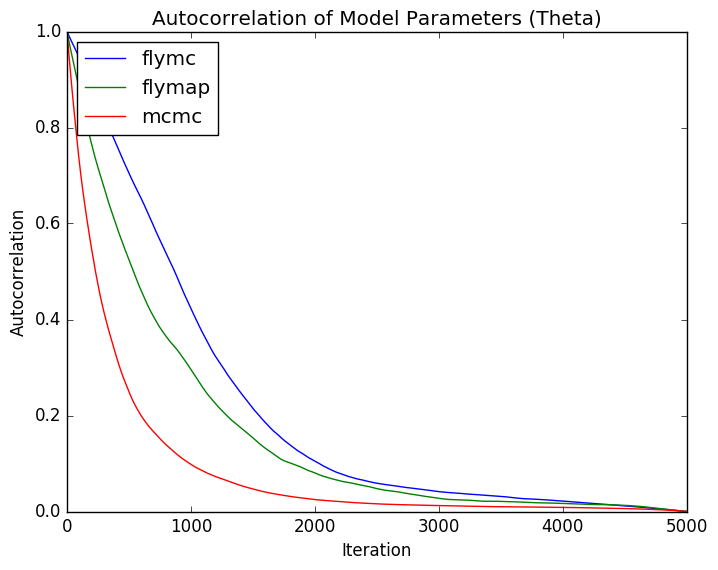
\includegraphics[scale=0.35]{Figures/final/logi_corr.png}
    \caption{Autocorrelation}
  \end{subfigure}
  \begin{subfigure}[t]{0.32\textwidth}
    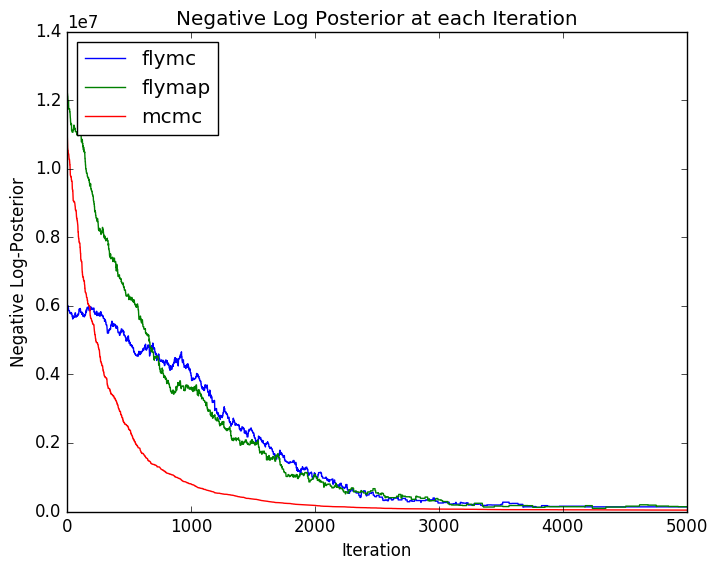
\includegraphics[scale=0.35]{Figures/final/logi_lik.png}
    \caption{Negative log posterior}
  \end{subfigure}
  \begin{subfigure}[t]{0.32\textwidth}
    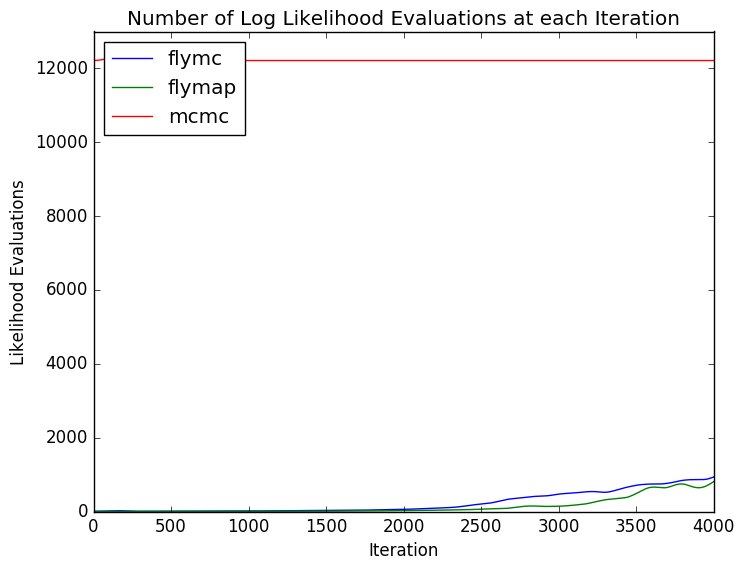
\includegraphics[scale=0.35]{Figures/final/logi_numlik.png}
    \caption{Number likelihood evaluations}
  \end{subfigure}
  \caption{Logistic regression binary classification on MNIST with MH-MCMC}
\end{figure}

\begin{figure}[htbp]
  \begin{subfigure}[t]{0.32\textwidth}
    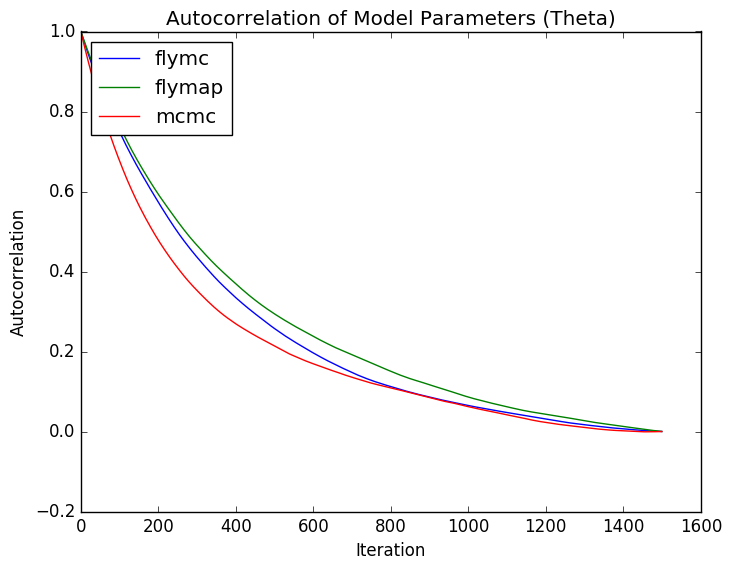
\includegraphics[scale=0.35]{Figures/final/soft_corr.png}
    \caption{Autocorrelation}
  \end{subfigure}
  \begin{subfigure}[t]{0.32\textwidth}
    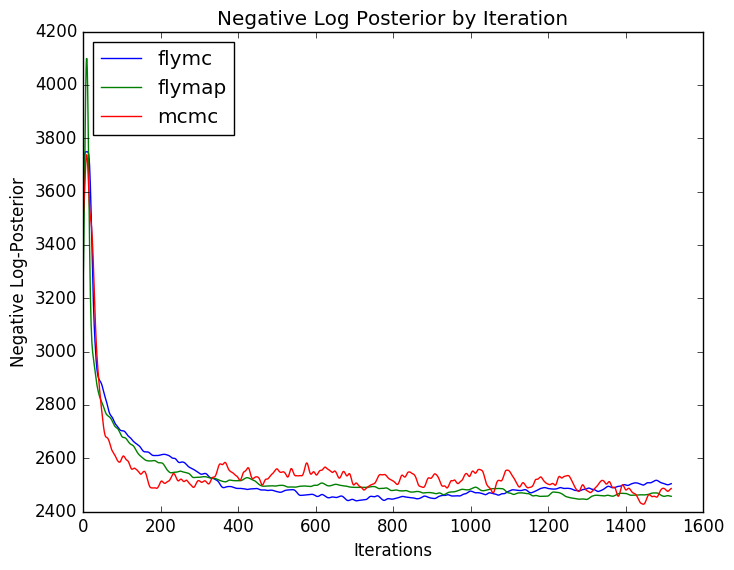
\includegraphics[scale=0.35]{Figures/final/soft_lik.png}
    \caption{Negative log posterior}
  \end{subfigure}
  \begin{subfigure}[t]{0.32\textwidth}
    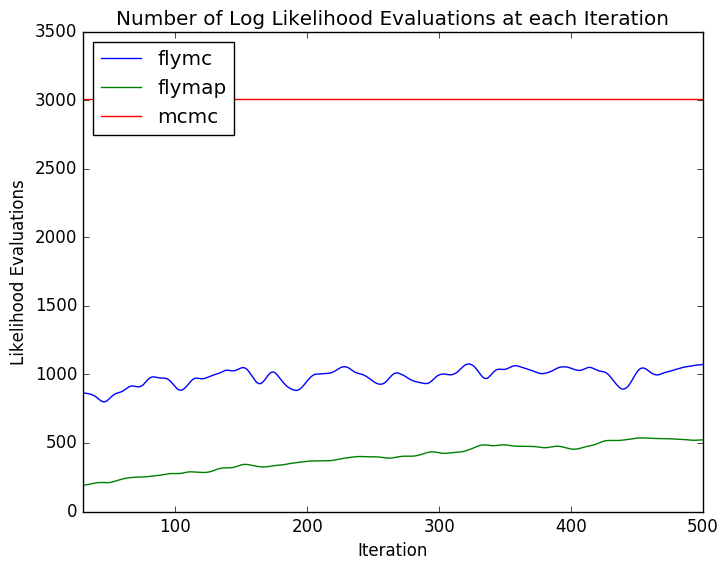
\includegraphics[scale=0.35]{Figures/final/soft_numlik.png}
    \caption{Number likelihood evaluations}
  \end{subfigure}
  \caption{Softmax 3-way classification on CIFAR-10 with Langevin dynamics}
\end{figure}

\begin{figure}[htbp]
  \begin{subfigure}[t]{0.32\textwidth}
    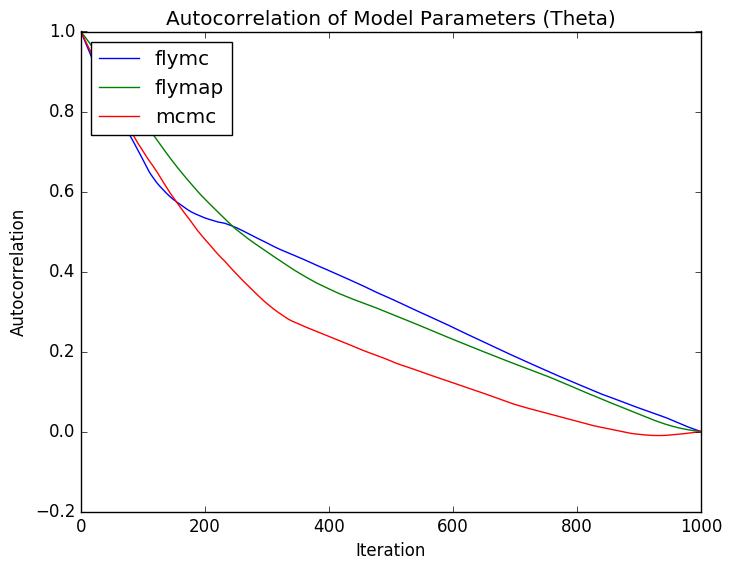
\includegraphics[scale=0.35]{Figures/final/reg_corr.png}
    \caption{Autocorrelation}
  \end{subfigure}
  \begin{subfigure}[t]{0.32\textwidth}
    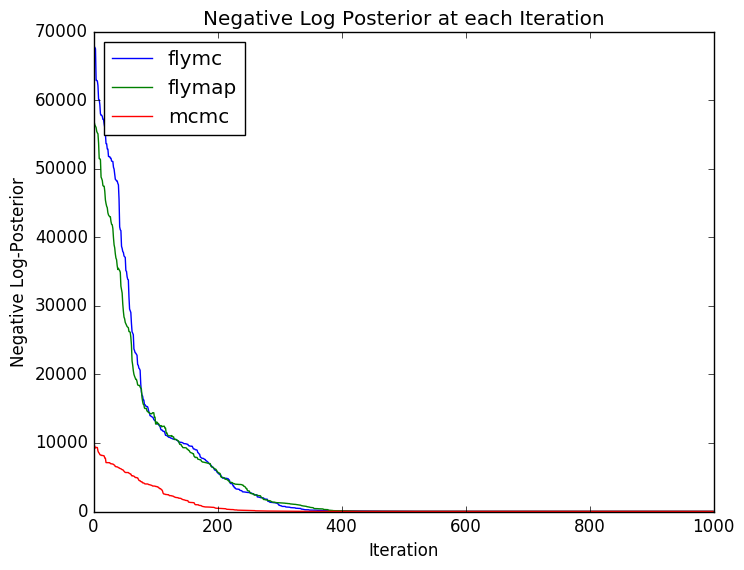
\includegraphics[scale=0.35]{Figures/final/reg_lik.png}
    \caption{Negative log posterior}
  \end{subfigure}
  \begin{subfigure}[t]{0.32\textwidth}
    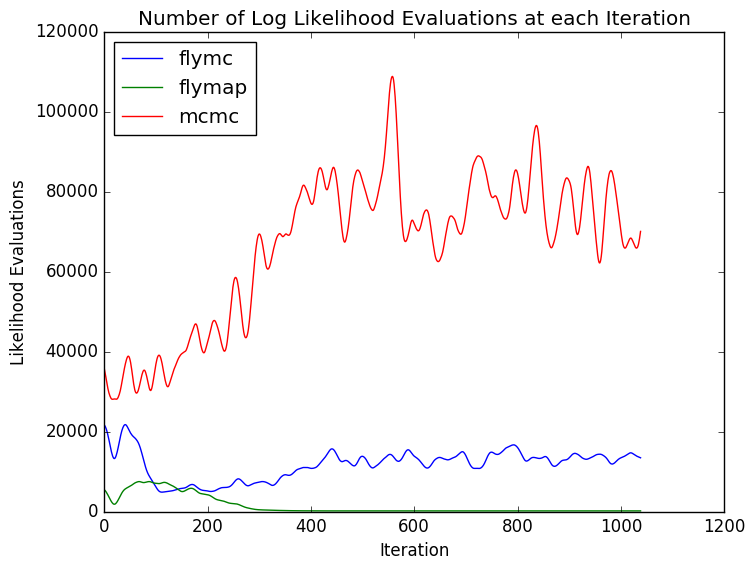
\includegraphics[scale=0.35]{Figures/final/reg_numlik.png}
    \caption{Number likelihood evaluations}
  \end{subfigure}
  \caption{Robust regression on synthesized data with slice sampler}
\end{figure}


\section{Conclusion }

%\todo{Write this section, make sure the mention extension work including: minimizing bound over posterior samples instead of MAP tuning (see  ```MAP-tuning the lower bound'')}

\textbf{You should end by critically evaluating your work and suggest
what you would have done given more time.}

From this practical, we learned that FlyMC is n elegant framework for MCMC sampling that can lead into speed-ups of an order of magnitude greater than what has been seen with conventional MCMC samplers. Map-tuning FlyMC, yielded the fastest samplers with effective sampling weights as low as 20 times that of traditional MCMC.

As a summary of the work undertaken, our practical implementation of Firefly MC led, which was based on the code provided by HIPs, led to several important pull requests on Github which fixed the caching of bright variables. in addition, we had to produce plots, tune parameters, and amend the sampling procedure so that they would work with the various kinds of  data that was investigated in the paper.

A thorough grounding  into the underpinning mathematical background of FlyMc was also given.

We replicated almost almost all the graphs and figures in  the paper, however, we would have liked to generate more tabulated data on effective sample rates than we could have.

Many extensions of the work we have presented are possible. One particularly
important experiment would be to tune the lower bounds over multiple parameter
values sampled from the posterior rather than the single MAP estimate. This
would ensure a low number of expected bright points, even if we are possibly
far away from the MAP estimate. Given the significant performance difference
% between MAP-tuned and untuned FlyMC, we expect
tuning lower bounds in this manner to yield even lower numbers of bright points
and hence greater speedups over traditional MCMC.

Another direction for investigation is on the lower bounds $B_n$. The
assumptions made in assumptions 1 and 2 on $B_n$ are required
for formulating FlyMC, and the authors do a good first pass discussion about
using exponential families for $B_n$. However, it may be interesting to
consider other functional forms for $B_n$ such that $\prod_{n=1}^N B_n(\theta)$
is cheap to compute. Furthermore, it is often the case that we are working with
likelihoods $L(\theta)$ which do not have a well-known lower bound (e.g.\
$L(\theta)$ could be parameterized by a deep neural network). In these
situations, one would like any form of lower bound which is non-zero. Alternatively,
one could investigate what happens when approximate bounds are used for $B_n(\theta)$
where cite the 0 <= Bn <= 1 does not hold for all $\theta$.

Finally, we would like to mention that although the motivation for this work
is computing on big datasets with large $N$, most experiments presented here
and in the paper were small and run on a single machine. For FlyMC to truly be
impactful in big data applications, an implementation on a distributed
computing platform (e.g.\ Spark, Hadoop) which demonstrates tractable MCMC on
large datacenter-scale datasets would be a convincing and immediately useful
line of work.


\bibliographystyle{alpha}
\nocite{*}
\bibliography{refs.bib}

\onecolumn

\end{document}
